\section{Problem Statement}
\label{sec:problem}

In this section we convert a human-path constraint into a multi-partite graph and formulate the informative path planning problem into a class of submodular orienteering on a multi-partite graph.

\subsection{Information maximization path planning}

Consider a discretized map of the world formed by a set of cells $ \mathbf{S}$ and suppose that the robot moves with constant speed from a cell to its neighbors.
In the search task, each cell in a discretized map is assigned an entropy value to represent the information distribution.
Because the robot's path must be connected, the robot's motion is constrained by a graph topology determined by the cell neighborhood. 
In a period of time of length $ T $, we denote the robot's path as $ X = [x_{1}, x_{2} , \cdots , x_{T}] $, and note that this path must satisfy the connection constraint on the discretized map.
We adopt an observation coverage model for the robot, which means that the robot can observe not only the cell it currently occupies but also neighboring cells within a given range.
Let the observation at time step $ t $ be $ O^{X}_{t} $, which describes both the observed cells and how well they are observed.
Thus the robot's path, $X$, induces a sequence of observations $ \mathbf{O}^{X} = \{ O^{X}_{1}, \cdots , O^{X}_{T-1}, O^{X}_{T} \}$.

We assume that the observation coverage model follows Bayes rule.
Thus we can define the information gain of the robot using mutual information $ I( \mathbf{S} \mid \mathbf{O}^{X} ) =  H( \mathbf{S} ) - H( \mathbf{S}, \mathbf{O}^{X}  ) $.
The entropy reduction over the problem space $ \mathbf{S} $ by the observation $ \mathbf{O}^{X} $ is the {\em information gain} to the robot.

\subsection{Human path constraint}

\begin{figure}[hbtp]
\centering
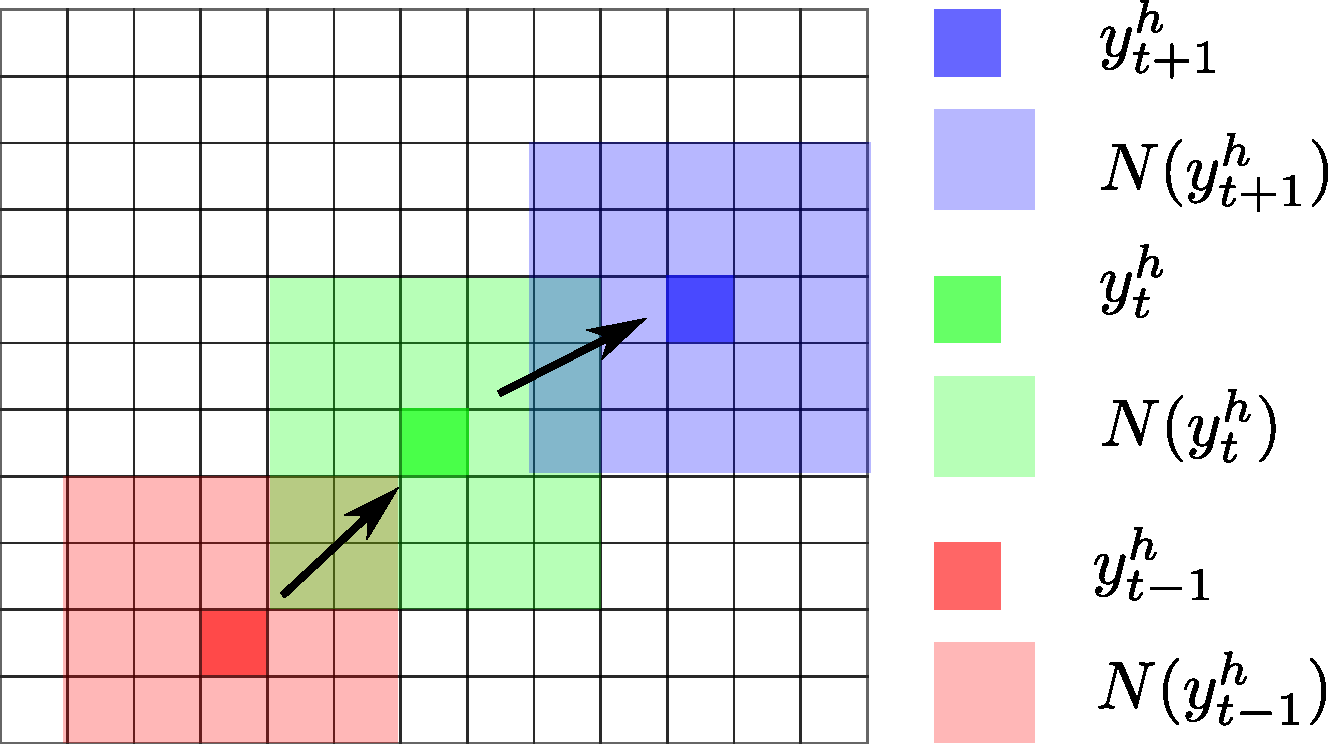
\includegraphics[width=0.6\linewidth]{./images/humanConstraint}
\caption{How the multi-partite graph is obtained.}
\label{fig:humanConstraint}
\end{figure}
%todo I thinkg you need to add more of the grid to the figure. It seems
%disconnected as it is.

As discussed in the introduction, there are several ways that a human can constrain the robot's path.
Without loss of generality, we adopt a ``wingman" approach and assume we have a model that can predict the human's path.
We denote the human's $T$-step path as $ Y^{h} = [y^{h}_{1}, y^{h}_{2} , \cdots , y^{h}_{T}] $.
We define a neighbor function $ N () $ that represents the assumption from the introduction that the robot can deviate from a constrained path by no more than a given tolerance.  
At each time step, this neighborhood induces the set of {\em visitable cells} for the robot, which is denoted by $ N( y^{h}_{t} ) $.
Figure \ref{fig:humanConstraint} gives an example.
By organizing the set of visitable cells at time $ t $ into a partition of vertices, we can construct a multi-partite graph $ G = (V, E, T) $ from the constrained path.
A partition $ V(t) \in V $ is obtained from the cells in $ N( y^{h}_{t} ) $.
The edge set $ E $ is determined by the neighborhood of each cell from the discretized map.

Imposing the path constraint $ Y^{h} $, we define the multi-partite graph as follows.
Figure \ref{fig:MultiPartite} illustrates how the path constraint induces the multi-partite graph for a notional human path.
Note that a cell in the discretized map might appear in multiple partitions due to overlaps between sets by $ N( y^{h}_{t} ) $ at different $ t $.

\begin{figure}[htbp]
\centering
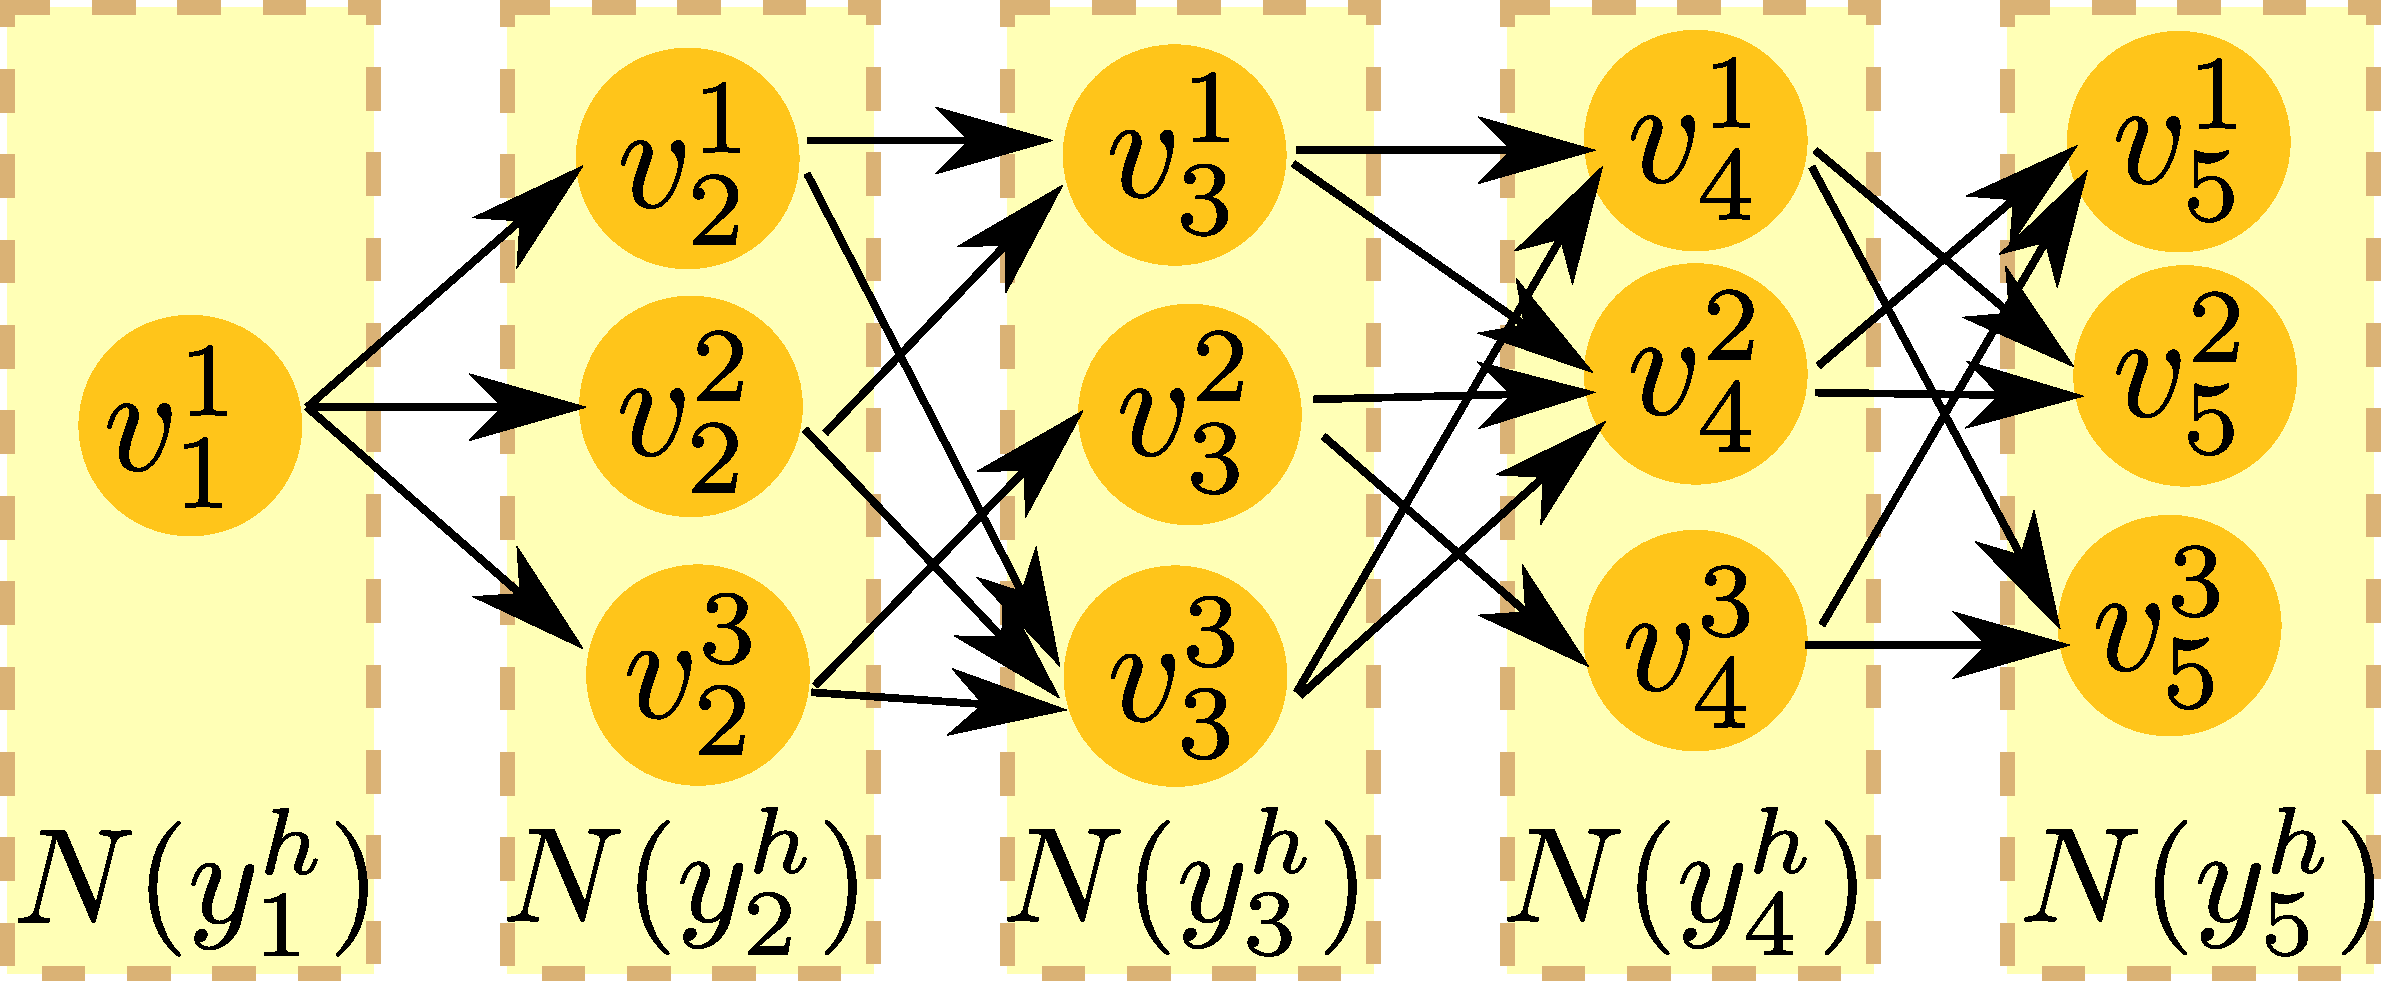
\includegraphics[width=0.6\linewidth]{./images/MultiPartite.pdf}
\caption{A multi-partite graph from a human path constraint.}
\label{fig:MultiPartite}
\end{figure}

\begin{mydef}[\textbf{Multi-Partite Graph}]
\label{def:multi_partite}
The multi-partite graph $ G = (V, E, T) $ is defined as a graph of $ T $ partitions. 
The vertex set $ V $ is defined as $ V = \cup_{t=1}^{T} V(t) $.
Each partition $ V(t) $ is a set of vertices $ v^{i}_{t} $, where $ t $ indicates which partition the vertex $ x $ is in and $ i $ indicates the index of this vertex.
Edges are directed, originating from vertices in set $ V(t) $ to vertices in set $ V(t+1) $.
Let $ v^{i}_{t} \in V(t) $ and $ v^{j}_{t+1} \in V(t+1) $.
A directed edge $ (v^{i}_{t}, v^{j}_{t+1}) $ connects vertices $ v^{i}_{t} $ and $ v^{j}_{t+1} $. 
\end{mydef}

In order to guarantee that the search process on a multi-partite graph $ G = (V, E, T) $ always ends with a path of length $ T $, we use a pruning process to ensure that each vertex can be reached from the previous partition and is connected to a vertex in the next partition.
The pruning process includes a forward pruning and a backward pruning.
The forward pruning traverses from partition $ V(2) $ to partition $ V(T) $ and removes any vertex that has no incoming edge; all edges incident to this vertex are also removed.
The backward pruning traverses from partition $ V(T-1) $ to partition $ V(1) $, and removes any vertex that has no outgoing edge; all edges incident to this vertex are also removed.

\subsection{The Optimization Problem Model}

Without loss of generality, we assume all paths start from the same vertex.
Thus, we have only one vertex in partition $ V(1) $, as illustrated in Figure \ref{fig:MultiPartite}.
Because the objective of the path-planning problem is to maximize mutual information, and because mutual information is a submodular function~\cite{singh2009efficient}, we find it convenient to shift from the bulky notation for mutual information, $ I(\mathbf{S}; \mathbf{O}^{X} ) $, to the more concise notation of a general submodular function,  $ f(X) $. 
Because the mutual information $ I(\mathbf{S}; \mathbf{O}^{X} ) $ is independent of the sequence of the vertices in a path, we write $ X $ as a set in $ f() $ for simplicity.
$ f() $ supports multiple vertices representing the same cell, which is like choosing same position multiple times in a sensor coverage placement problem. 
%todo do we need this here? we say it below too

The objective of the search task is to maximize information gain subject to the path constraint.  Since the path constraint is encoded as the multi-partite graph, we can restate the objective as maximizing information gain on the multi-partite graph.
This yields a submodular orienteering problem on a multi-partite graph $ G = (V, E, T) $, which is given as

\begin{equation}
\label{eq:gnr_obj}
\begin{aligned}
Objective: & X^{*} = \underset{X}{\arg\max} f(X); \\
Constraint: & |X| = T, x_{t} \in V(t), (x_{t}, x_{t+1}) \in E.
\end{aligned}
\end{equation}

Exhaustive search could find the optimal path but the time-complexity of such a search makes this unacceptable in all problems except in small problems.
A greedy search is efficient but the performance of greedy search on a submodular problem is not guaranteed given a topological constraint~\cite{krause2012submodular}.
Instead of a greedy heuristic, we develop an alternative heuristic based on the property of mutual information.

Mutual information has two desirable properties that we exploit.  First, it is independent of the sequence of vertices on a path and, second, it follows a chain rule.  This chain rule property can be written as
$ f(x_{1}, x_{2}, \cdots , x_{T}) = f(x_{1}) + f(x_{2} \mid x_{1}) + 
\cdots + f(x_{T} \mid x_{1}, \cdots , x_{T-1}) $,
which yields a structured Bellman-like equation  
$ \hat{x}_{t} = \arg \max_{X_{t}} [ f(x_{t} \mid x_{1} , \cdots , x_{t-1}) + \max_{X_{t+1}, \cdots , X_{T}} f(x_{t+1}, \cdots , x_{T} \mid x_{1}, \cdots , x_{t}) ] $.
These structures lead to two key terms: \emph{maximum future reward} and \emph{maximum total reward}.

\begin{mydef}[\textbf{Maximum Future Reward}]
\label{def:max_future_reward}
Define the maximum future reward as
\begin{equation}
\nonumber
\label{eq:def_h}
h(x_{1} , \cdots, x_{t'} ) = \max_{V(t'+1), \cdots , V(T)} f(x_{t'+1}, \cdots x_{T} \mid x_{1}, \cdots , x_{t'}),
\end{equation} 
given the topology constraint
$ \forall \tau \in \{ t'+1 , \cdots , T \},  x_{\tau} \in V(\tau) $
and
$ \forall \tau \in \{ t'+2, \cdots ,T-1 \}, ( x_{\tau-1}, x_{\tau} ) \in E $.
\end{mydef}

\begin{mydef}[\textbf{Maximum Total Reward}]
\label{def:max_total_reward}
Define the maximum total reward from choosing $ x_{t} $ after $ x_{1} \cdots , x_{t'} $ have been chosen as, $ \forall t > t' $,
\begin{equation}
\nonumber
\label{eq:def_p_0}
\begin{aligned}
u(x_{t} \mid x_{1} , \cdots , x_{t'} ) = f(x_{t} \mid x_{1} , \cdots , x_{t'}) +  h( x_{1}, \cdots , x_{t'}, x_{t} ).
\end{aligned}
\end{equation}
\end{mydef}

If we could obtain the values $ u(x_{t} \mid x_{1} , \cdots , x_{t'} ) $, then we could greedily chose values for $\hat{x}_t$ as those that maximize $u()$ ; this would yield an optimal solution as $\hat{x}_t \to x_t $.  Unfortunately, the calculation on $ u(x_{t} \mid x_{1} , \cdots , x_{t'} ) $ is hard due to the submodularity of $f()$ and the topology constraint.
In the next section, we present a heuristic for $u()$ that yields good performance in empirical studies.
